% Created 2019-04-01 lun 10:34
% Intended LaTeX compiler: pdflatex
\documentclass[xcolor={usenames,svgnames,dvipsnames}]{beamer}
\usepackage[utf8]{inputenc}
\usepackage[T1]{fontenc}
\usepackage{graphicx}
\usepackage{grffile}
\usepackage{longtable}
\usepackage{wrapfig}
\usepackage{rotating}
\usepackage[normalem]{ulem}
\usepackage{amsmath}
\usepackage{textcomp}
\usepackage{amssymb}
\usepackage{capt-of}
\usepackage{hyperref}
\usepackage{color}
\usepackage{listings}
\usepackage{mathpazo}
\usepackage{gensymb}
\usepackage{amsmath}
\usepackage{esdiff}
\usepackage{steinmetz}
\bibliographystyle{plain}
\usepackage[emulate=units]{siunitx}
\sisetup{fraction=nice, decimalsymbol=comma, retain-unity-mantissa = false}
\newunit{\wattpeak}{Wp}
\newunit{\watthour}{Wh}
\newunit{\amperehour}{Ah}
\hypersetup{colorlinks=true, linkcolor=Blue, urlcolor=Blue}
\renewcommand{\thefootnote}{\fnsymbol{footnote}}
\beamertemplatenavigationsymbolsempty
\setbeamertemplate{footline}[frame number]
\newcommand{\laplace}[1]{\mathbf{#1}(\mathbf{s})}
\newcommand{\slp}{\mathbf{s}}
\newcommand{\fasor}[1]{\mathbf{#1}(\omega)}
\newcommand{\atan}{\mathrm{atan}}
\AtBeginSection[]{\begin{frame}[plain]\tableofcontents[currentsection,hideallsubsections]\end{frame}}
\setbeamercolor{alerted text}{fg=blue!50!black} \setbeamerfont{alerted text}{series=\bfseries}
\usetheme[hideothersubsections]{Boadilla}
\usecolortheme{rose}
\usefonttheme{serif}
\author{Oscar Perpiñán Lamigueiro}
\date{Abril 2019}
\title{Acoplamientos Magnéticos}
\subtitle{Teoría de Circuitos II}
\hypersetup{
 pdfauthor={Oscar Perpiñán Lamigueiro},
 pdftitle={Acoplamientos Magnéticos},
 pdfkeywords={},
 pdfsubject={},
 pdfcreator={Emacs 26.1 (Org mode 9.2)}, 
 pdflang={Spanish}}
\begin{document}

\maketitle

\section{Bobina}
\label{sec:org1fdc5e0}

\begin{frame}[label={sec:orge4ab99d}]{Ley de Ampere}
Una corriente eléctrica circulando por un conductor crea un campo magnético en torno al conductor (\emph{regla de la mano derecha})

\begin{center}
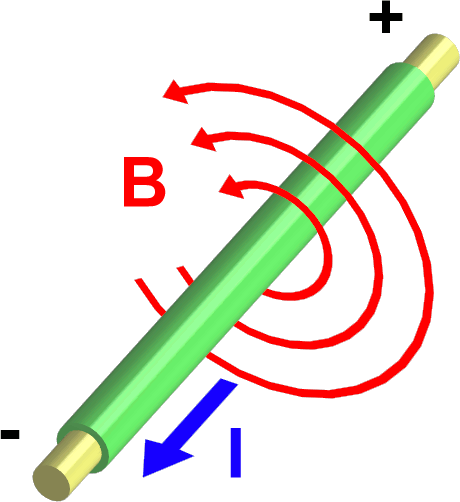
\includegraphics[height=0.7\textheight]{figs/Electromagnetism.png}
\end{center}
\end{frame}


\begin{frame}[label={sec:orgcb1f78b}]{Ley de Faraday}
Cuando un \alert{campo magnético variable} atraviesa una espira \alert{estática} aparece una \alert{tensión inducida} \alert{proporcional al flujo} y opuesta a su variación.

\[
u(t) = \frac{\mathrm{d}\phi}{\mathrm{d}t} 
\]

El flujo magnético es la cantidad de líneas de fuerza magnética que atraviesan una superficie. 

\begin{columns}
\begin{column}{0.3\columnwidth}
\[
\phi = \vec{B} \cdot \vec{A} \ [\mathrm{Wb}]
\]
\end{column}

\begin{column}{0.7\columnwidth}
\begin{center}
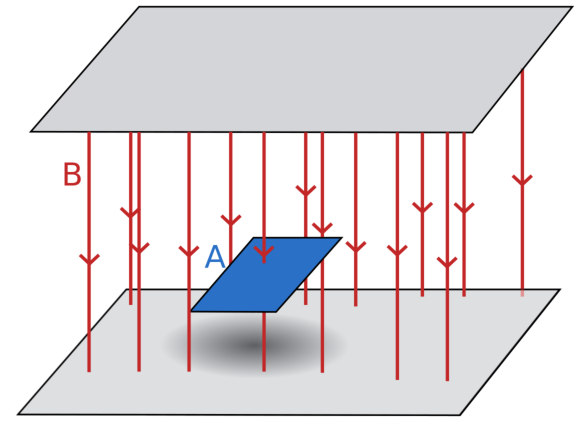
\includegraphics[height=0.45\textheight]{figs/flujo_magnetico.pdf}
\end{center}
\end{column}
\end{columns}
\end{frame}

\begin{frame}[label={sec:orgb792fc2}]{Bobina}
Una bobina es un arrollamiento de un conductor (\emph{conjunto de \(N\) espiras conectadas en serie}) alrededor de un material ferromagnético:
\begin{itemize}
\item Al circular corriente se produce un campo magnético.
\item Este campo magnético atraviesa la propia bobina y produce una tensión (auto)inducida.
\end{itemize}
\begin{center}
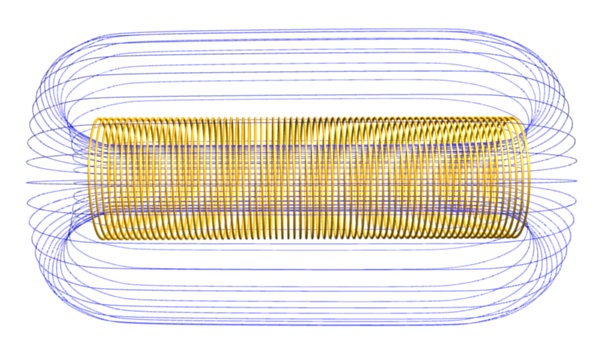
\includegraphics[height=0.5\textheight]{figs/Solenoide.jpg}
\end{center}
\end{frame}

\begin{frame}[label={sec:org1ca188b}]{Bobina}
\begin{itemize}
\item Tensión inducida en \(N\) espiras
\end{itemize}
\[
u(t) = N \cdot \frac{\mathrm{d}\phi(t)}{\mathrm{d} t}
\]
\begin{itemize}
\item En un circuito magnético lineal el flujo es proporcional a la corriente
\end{itemize}
\[
  \frac{\mathrm{d}\phi(t)}{\mathrm{d} i(t)} = \frac{\phi(t)}{i(t)}
\rightarrow
u(t) = N \cdot \frac{\phi(t)}{i(t)} \cdot \frac{\mathrm{d}i(t)}{\mathrm{d} t}
\]

\begin{itemize}
\item Autoinductancia (\(L\), [H])
\end{itemize}
\begin{columns}
\begin{column}{0.5\columnwidth}
\[
  \boxed{L = N \cdot \frac{\phi(t)}{i(t)}}
\]
\[
  \boxed{u(t) = L \cdot \frac{\mathrm{d}i(t)}{\mathrm{d} t}}
\]
\end{column}
\begin{column}{0.5\columnwidth}
\begin{center}
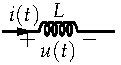
\includegraphics[height=0.2\textheight]{figs/Bobina.pdf}
\end{center}
\end{column}
\end{columns}
\end{frame}
\section{Acoplamiento magnético}
\label{sec:org2bd5032}
\begin{frame}[label={sec:org8c40340},plain]{}
\begin{center}
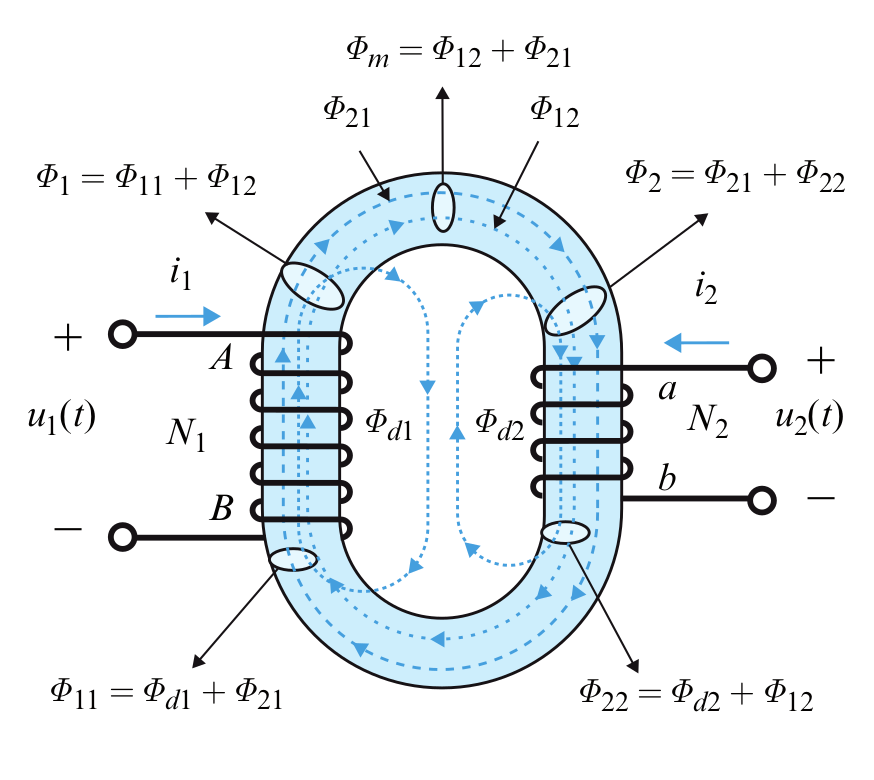
\includegraphics[height=0.8\textheight]{figs/Acoplamiento1.png}
\end{center}

\(\Phi_{ii}\): flujo producido por la bobina \(i\)

\(\Phi_{ij}\): flujo recibido en bobina \(i\) producido por bobina \(j\)

\(\Phi_{i}\): flujo total que atraviesa la bobina \(i\)
\end{frame}
\begin{frame}[label={sec:orgcc0b447},plain]{}
\begin{columns}
\begin{column}{0.5\columnwidth}
\begin{align*}
  u_1(t) = &N_1 \frac{\mathrm{d}\phi_1}{\mathrm{d}t} = \\
  &N_1 \frac{\mathrm{d}\phi_{11}}{\mathrm{d}t} + N_1 \frac{\mathrm{d}\phi_{12}}{\mathrm{d}t}
\end{align*}
\end{column}

\begin{column}{0.5\columnwidth}
\begin{align*}
  u_2(t) = &N_2 \frac{\mathrm{d}\phi_2}{\mathrm{d}t} = \\
  &N_2 \frac{\mathrm{d}\phi_{22}}{\mathrm{d}t} + N_2 \frac{\mathrm{d}\phi_{21}}{\mathrm{d}t}
\end{align*}
\end{column}
\end{columns}

\begin{center}
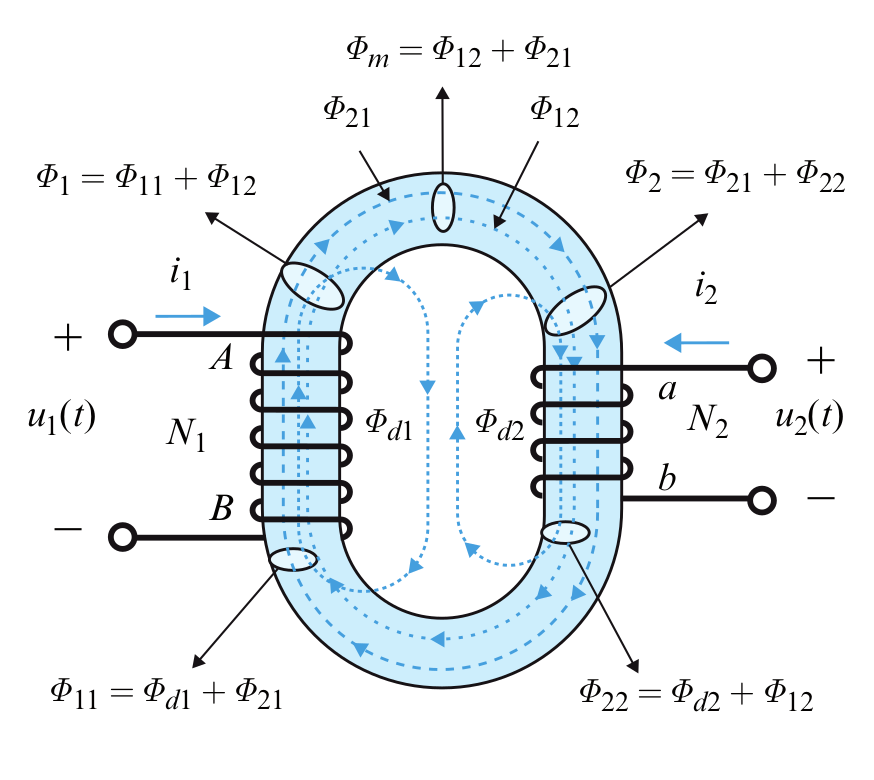
\includegraphics[height=0.65\textheight]{figs/Acoplamiento1.png}
\end{center}

\begin{center}
\(\Phi_{ij}\): flujo recibido en bobina \(i\) producido por bobina \(j\)
\end{center}
\end{frame}
\begin{frame}[label={sec:org79aea4b},plain]{}
\begin{columns}
\begin{column}{0.5\columnwidth}
\[
  L_1 = N_1 \frac{\phi_{11}}{i_1}
\]
\[
  M_{12} = N_1 \frac{\phi_{12}}{i_2}
\]
\end{column}
\begin{column}{0.5\columnwidth}
\[
  L_2 = N_2 \frac{\phi_{22}}{i_2}
\]
\[
  M_{21} = N_2 \frac{\phi_{21}}{i_1}
\]
\end{column}
\end{columns}

\begin{center}
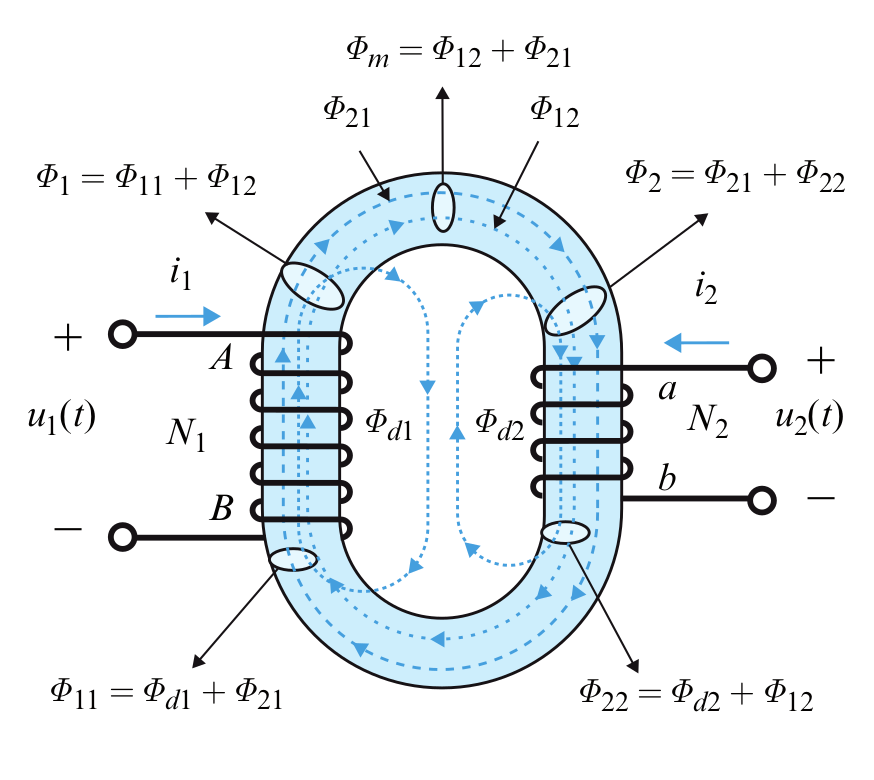
\includegraphics[height=0.65\textheight]{figs/Acoplamiento1.png}
\end{center}

\begin{center}
\(\Phi_{ij}\): flujo recibido en bobina \(i\) producido por bobina \(j\)
\end{center}
\end{frame}

\begin{frame}[label={sec:orga4c712f}]{Coeficiente de acoplamiento magnético}
\begin{center}
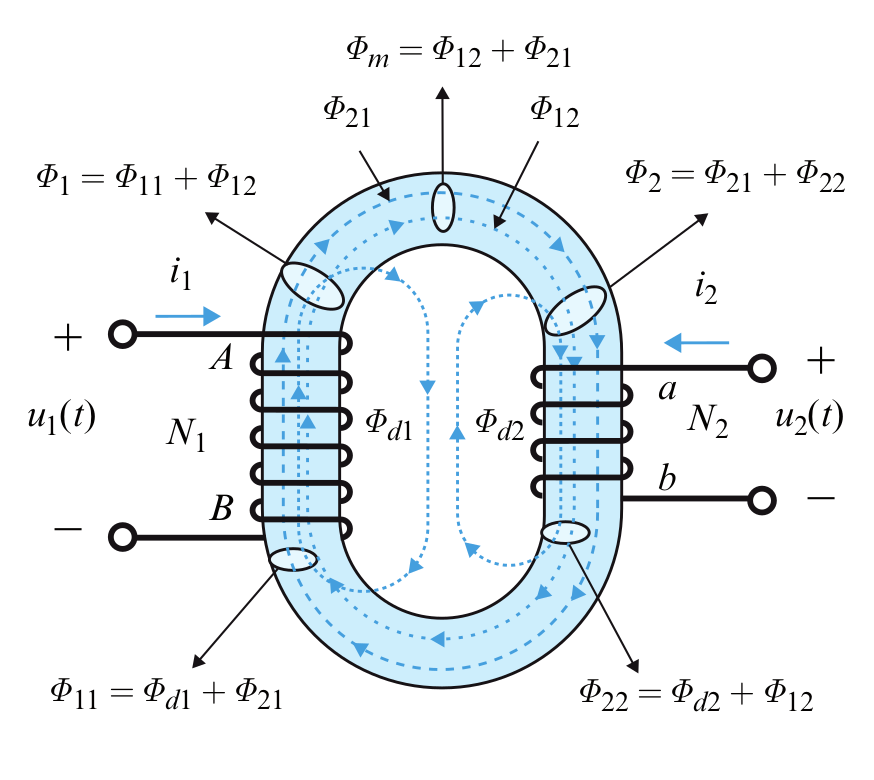
\includegraphics[height=0.58\textheight]{figs/Acoplamiento1.png}
\end{center}

\[
  k_{21} = \frac{\phi_{21}}{\phi_{11}} = 1 - \frac{\phi_{d1}}{\phi_{11}} \leq 1
\]

\[
  k_{12} = \frac{\phi_{12}}{\phi_{22}} = 1 - \frac{\phi_{d2}}{\phi_{22}} \leq 1
\]
\end{frame}



\begin{frame}[label={sec:orge45a45a}]{Coeficiente de inducción mutua}
\begin{itemize}
\item Mediante un balance energético puede demostrarse que:
\end{itemize}
\[
  M_{12} = M_{21} = M
\]

\[
  k_{12} = k_{21} = k
\]

\[
  \boxed{M = k \sqrt{L_1 \cdot L_2}} \qquad  k \leq 1
\]

\begin{itemize}
\item Cuando el acoplamiento entre las dos bobinas es perfecto:
\end{itemize}

\[\left.
\begin{array}{cc}
  \phi_{d1} = 0 \rightarrow   \phi_{11} = \phi_{21}\\
  \phi_{d2} = 0 \rightarrow \phi_{22} = \phi_{12} 
  \end{array} \right\} \rightarrow k = 1
\]
\end{frame}

\begin{frame}[label={sec:orgaad0a13}]{Resumen}
\[
  L_1 = N_1 \frac{\phi_{11}}{i_1}
\]

\[
  L_2 = N_2 \frac{\phi_{22}}{i_2}
\]


\begin{align*}
  M &= N_1 \frac{\phi_{12}}{i_2}\\
    &= N_2 \frac{\phi_{21}}{i_1}
\end{align*}

\[
  M = k \sqrt{L_1 \cdot L_2}
\]
\end{frame}

\section{Representación Circuital}
\label{sec:org57596c8}
\begin{frame}[label={sec:org7586d4f}]{Flujos del mismo sentido}
\begin{columns}
\begin{column}{0.5\columnwidth}
\begin{center}
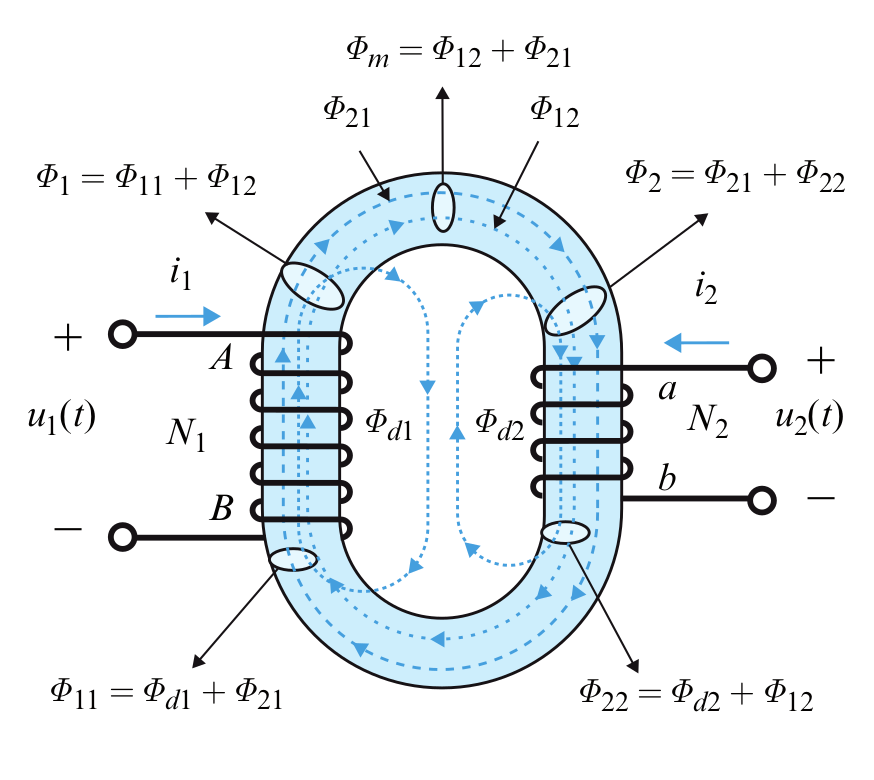
\includegraphics[width=.9\linewidth]{figs/Acoplamiento1.png}
\end{center}
\end{column}

\begin{column}{0.5\columnwidth}
\begin{center}
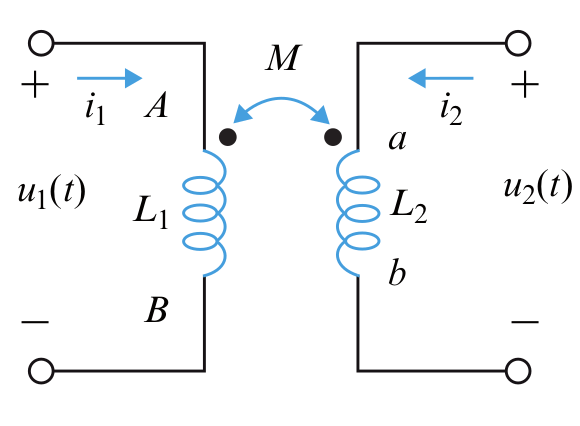
\includegraphics[width=.9\linewidth]{figs/Acoplamiento1_circuito.png}
\end{center}
\end{column}
\end{columns}

\alert{Convención del punto}: se señala con un punto los terminales de las
bobinas por los que hay que introducir corrientes que producen flujos
del mismo sentido. Una corriente que entra por un terminal con punto
induce una tensión positiva en el otro terminal con punto.
\end{frame}
\begin{frame}[label={sec:org61b823a}]{Flujos del mismo sentido}
\begin{columns}
\begin{column}{0.5\columnwidth}
\begin{center}
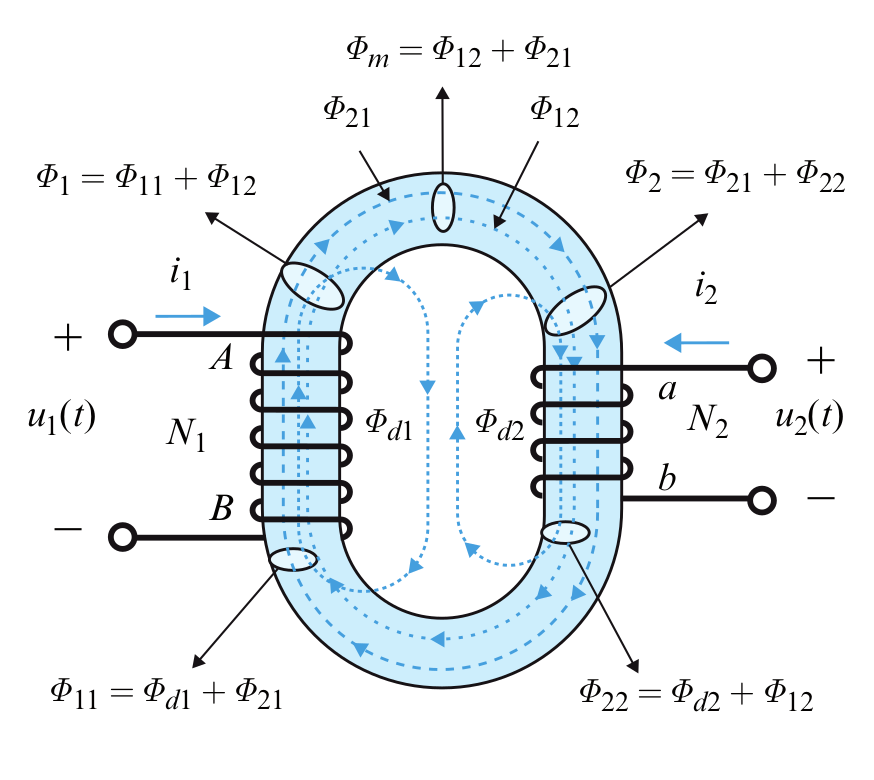
\includegraphics[width=.9\linewidth]{figs/Acoplamiento1.png}
\end{center}
\end{column}

\begin{column}{0.5\columnwidth}
\begin{center}
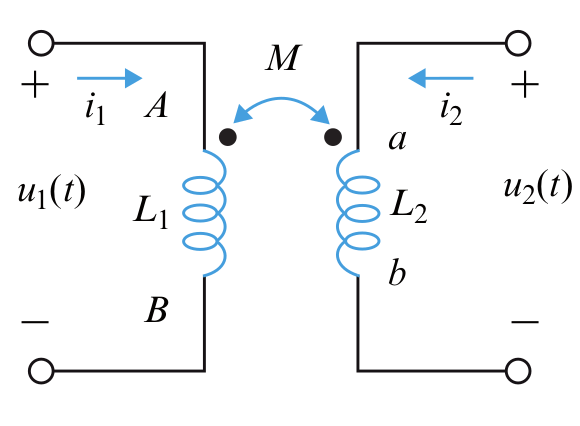
\includegraphics[width=.9\linewidth]{figs/Acoplamiento1_circuito.png}
\end{center}
\end{column}
\end{columns}

\begin{align*}
  u_1(t) &= L_1 \frac{\mathrm{d}i_1(t)}{\mathrm{d}t} + M \frac{\mathrm{d}i_2(t)}{\mathrm{d}t}\\
  u_2(t) &= M \frac{\mathrm{d}i_1(t)}{\mathrm{d}t} + L_2 \frac{\mathrm{d}i_2(t)}{\mathrm{d}t}
\end{align*}
\end{frame}
\begin{frame}[label={sec:org23401c7}]{Flujos contrapuestos}
\begin{center}
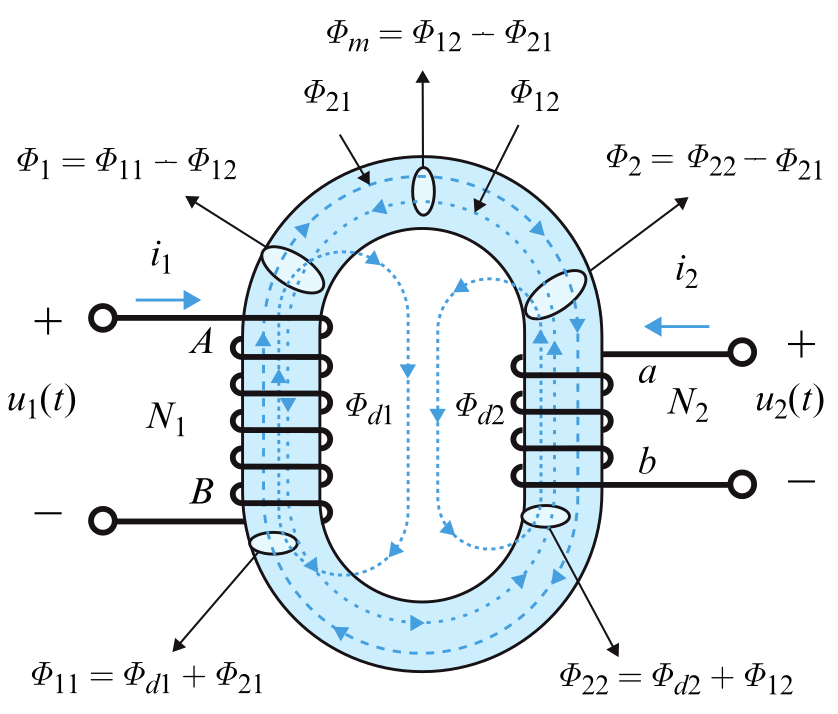
\includegraphics[height=0.9\textheight]{figs/Acoplamiento2.png}
\end{center}

Las corrientes \(i_1\) e \(i_2\) producen flujos de sentido contrario.
\end{frame}
\begin{frame}[label={sec:orgcafe3e8}]{Representación Circuital}
\begin{columns}
\begin{column}{0.5\columnwidth}
\begin{center}
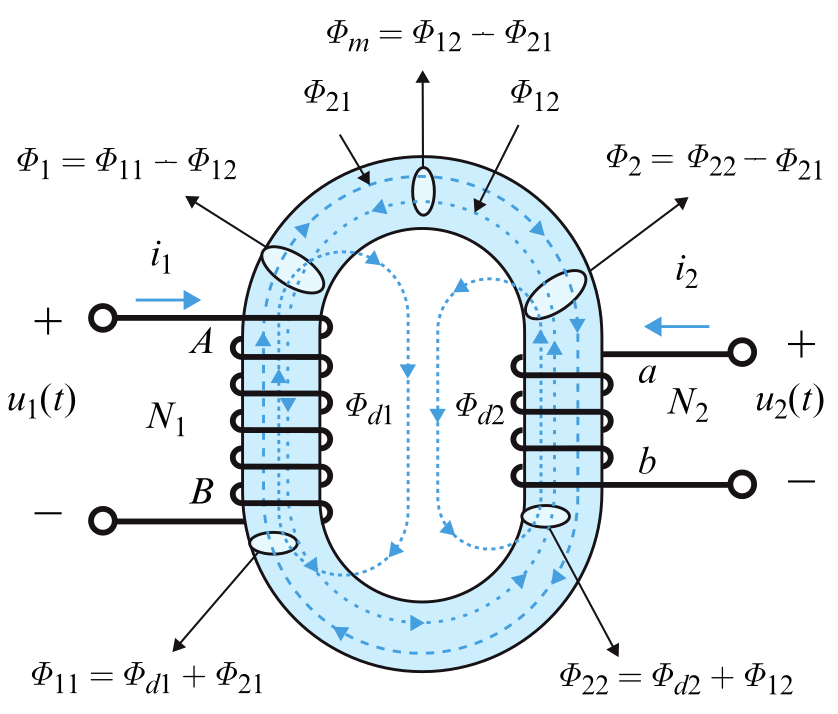
\includegraphics[height=0.45\textheight]{figs/Acoplamiento2.png}
\end{center}
\end{column}

\begin{column}{0.5\columnwidth}
\begin{center}
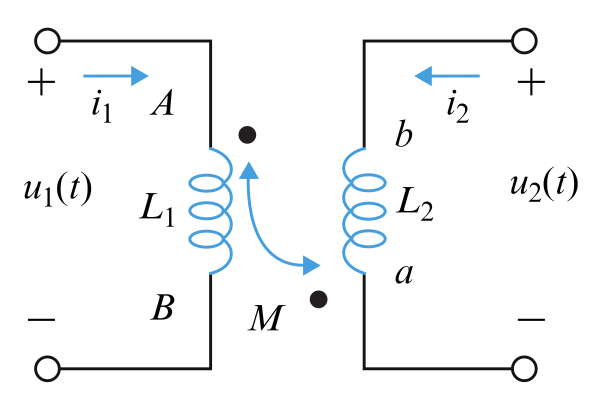
\includegraphics[height=0.45\textheight]{figs/Acoplamiento2_circuito.png}
\end{center}
\end{column}
\end{columns}
\alert{Convención del punto}: se señala con un punto los terminales de las
bobinas por los que hay que introducir corrientes que producen flujos
del mismo sentido. Una corriente que entra por un terminal con punto
induce una tensión positiva en el otro terminal con punto.
\end{frame}
\begin{frame}[label={sec:org8f01d7a}]{Representación Circuital}
\begin{columns}
\begin{column}{0.5\columnwidth}
\begin{center}
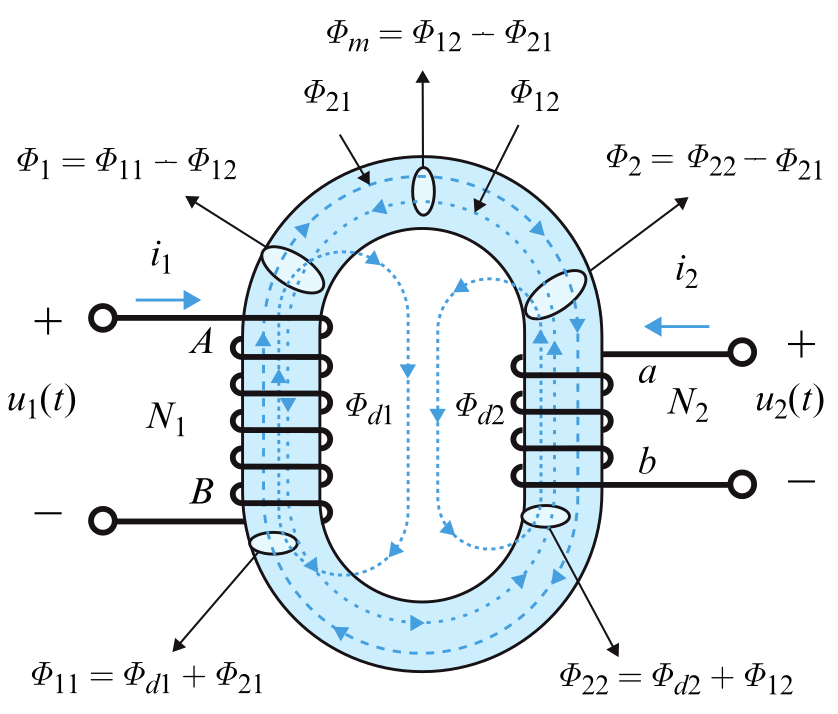
\includegraphics[height=0.45\textheight]{figs/Acoplamiento2.png}
\end{center}
\end{column}

\begin{column}{0.5\columnwidth}
\begin{center}
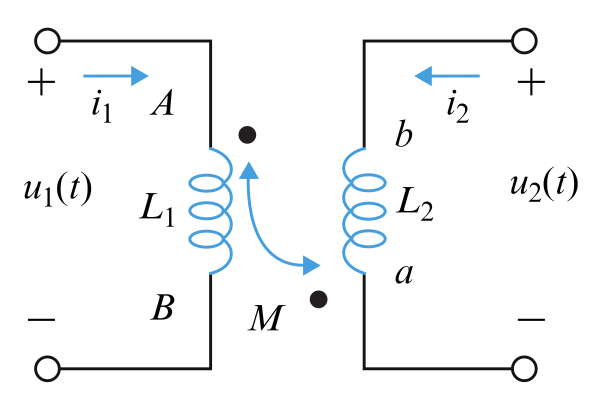
\includegraphics[height=0.45\textheight]{figs/Acoplamiento2_circuito.png}
\end{center}
\end{column}
\end{columns}
\begin{align*}
  u_1(t) &= L_1 \frac{\mathrm{d}i_1(t)}{\mathrm{d}t} - M \frac{\mathrm{d}i_2(t)}{\mathrm{d}t}\\
  u_2(t) &= - M \frac{\mathrm{d}i_1(t)}{\mathrm{d}t} + L_2 \frac{\mathrm{d}i_2(t)}{\mathrm{d}t}
\end{align*}
\end{frame}
\begin{frame}[label={sec:orgfdb5351}]{Criterio del punto}
\begin{center}
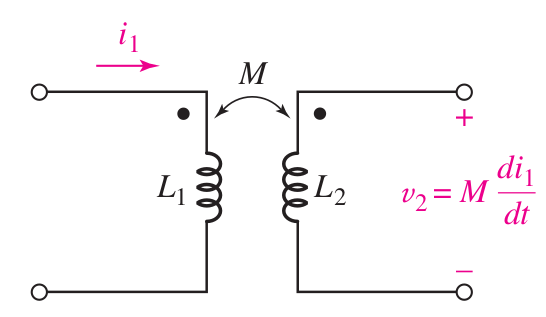
\includegraphics[width=.9\linewidth]{figs/punto1.png}
\end{center}
\end{frame}

\begin{frame}[label={sec:org7c327e6}]{Criterio del punto}
\begin{center}
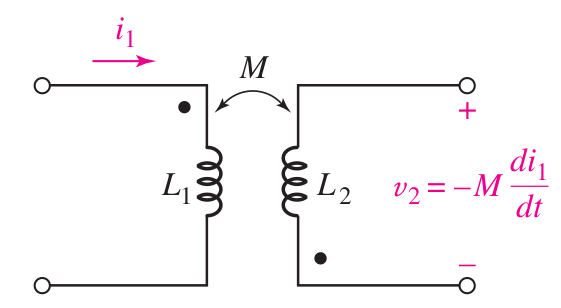
\includegraphics[width=.9\linewidth]{figs/punto2.png}
\end{center}
\end{frame}

\begin{frame}[label={sec:org0cedcf0}]{Criterio del punto}
\begin{center}
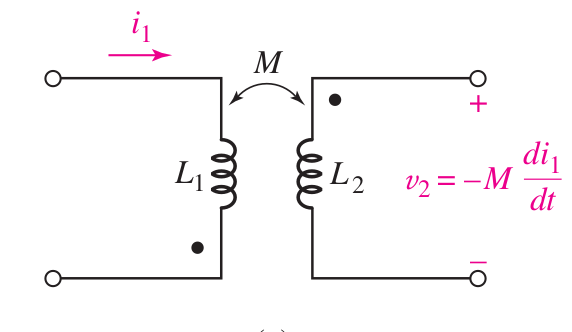
\includegraphics[width=.9\linewidth]{figs/punto3.png}
\end{center}
\end{frame}
\begin{frame}[label={sec:orgb489ea9}]{Criterio del punto}
\begin{center}
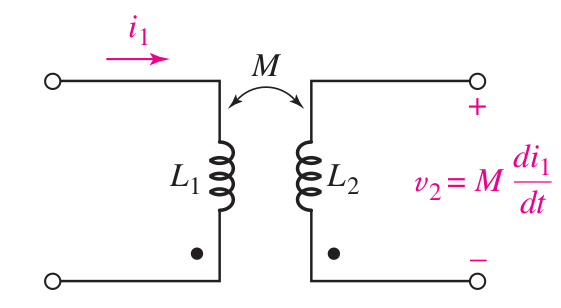
\includegraphics[width=.9\linewidth]{figs/punto4.png}
\end{center}
\end{frame}
\begin{frame}[label={sec:org409ff05}]{Corriente Alterna Sinusoidal}
\begin{columns}
\begin{column}{0.5\columnwidth}
\begin{center}
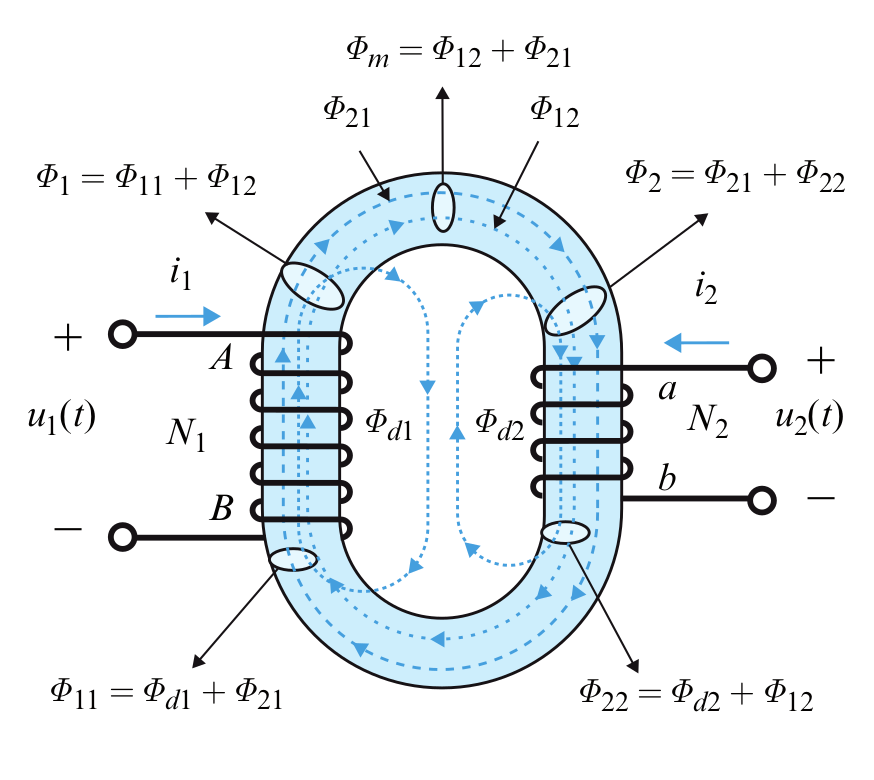
\includegraphics[height=0.45\textheight]{figs/Acoplamiento1.png}
\end{center}
\end{column}

\begin{column}{0.5\columnwidth}
\begin{center}
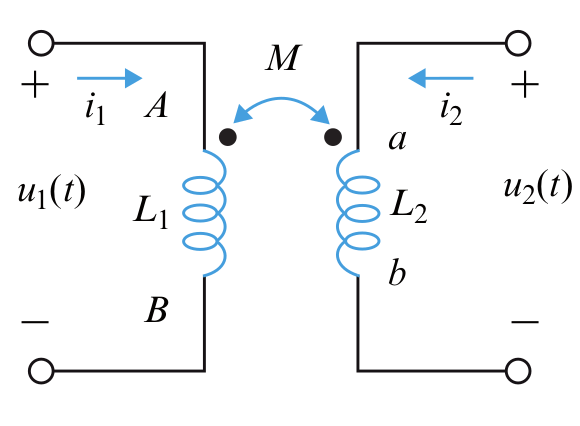
\includegraphics[height=0.45\textheight]{figs/Acoplamiento1_circuito.png}
\end{center}
\end{column}
\end{columns}
\begin{align*}
  \overline{U}_1 &= j \omega L_1 \overline{I}_1 + j \omega M \overline{I}_2\\
  \overline{U}_2 &= j \omega M \overline{I}_1 + j \omega L_2 \overline{I}_2
\end{align*}
\end{frame}
\begin{frame}[label={sec:org81fd55d}]{Corriente Alterna Sinusoidal}
\begin{columns}
\begin{column}{0.5\columnwidth}
\begin{center}
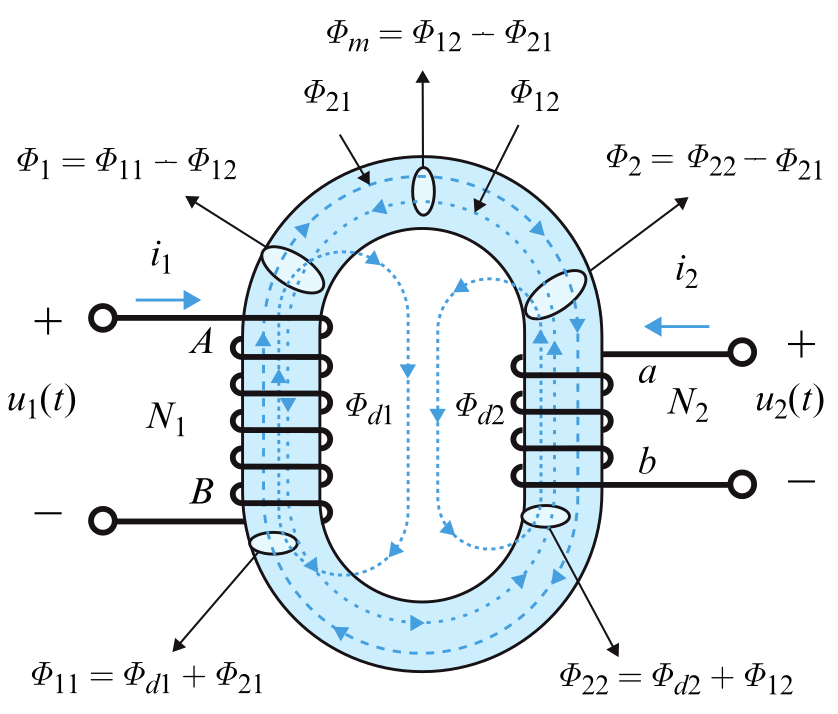
\includegraphics[height=0.45\textheight]{figs/Acoplamiento2.png}
\end{center}
\end{column}

\begin{column}{0.5\columnwidth}
\begin{center}
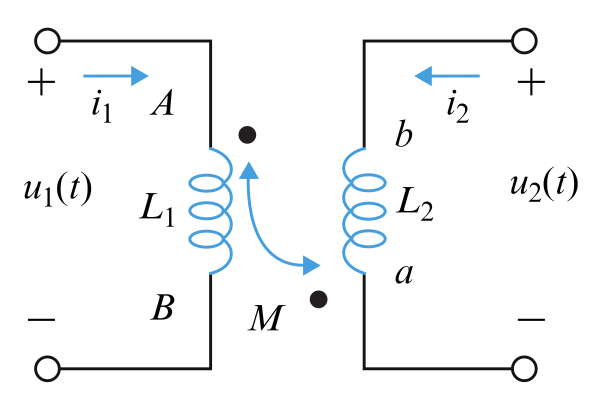
\includegraphics[height=0.45\textheight]{figs/Acoplamiento2_circuito.png}
\end{center}
\end{column}
\end{columns}
\begin{align*}
  \overline{U}_1 &= j \omega L_1 \overline{I}_1 - j \omega M \overline{I}_2\\
  \overline{U}_2 &= - j \omega M \overline{I}_1 + j \omega L_2 \overline{I}_2
\end{align*}
\end{frame}
\begin{frame}[label={sec:org5ac560c}]{Ejemplo: acoplamiento de bobinas en serie}
\begin{center}
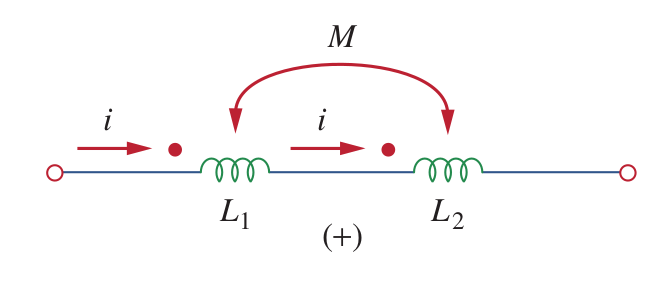
\includegraphics[width=.9\linewidth]{figs/bobinas_serie1.png}
\end{center}
\[
  \overline{U}_1 = (j \omega L_1 + j \omega M) \overline{I}
\]

\[
  \overline{U}_2 = (j \omega L_2 + j \omega M) \overline{I}
\]

\[
 \overline{U} = \overline{U}_1 + \overline{U}_2 \rightarrow \boxed{L = L_1 + L_2 + 2M}
\]
\end{frame}
\begin{frame}[label={sec:org0bda34d}]{Ejemplo: acoplamiento de bobinas en serie}
\begin{center}
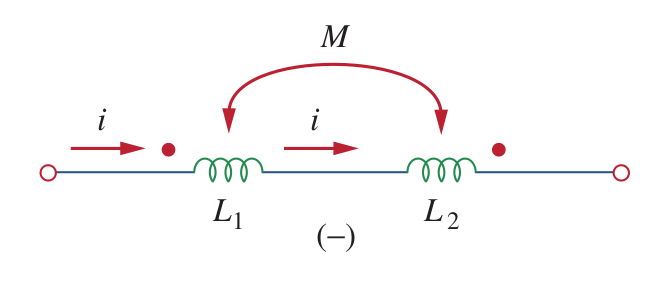
\includegraphics[width=.9\linewidth]{figs/bobinas_serie2.png}
\end{center}
\[
  \overline{U}_1 = (j \omega L_1 - j \omega M) \overline{I}
\]

\[
  \overline{U}_2 = (j \omega L_2 - j \omega M) \overline{I}
\]

\[
 \boxed{L = L_1 + L_2 - 2M}
\]
\end{frame}
\end{document}